\documentclass{article}

% Colors
\usepackage[dvipsnames]{xcolor}

% Basics
\usepackage[margin=1in]{geometry}
\usepackage{amsmath, amssymb, amsthm}
\usepackage{enumitem}
\usepackage{mathtools}
\usepackage{cancel}

% Figures
\usepackage{tikz}
\usetikzlibrary{arrows.meta, positioning, calc, shapes.geometric, angles, quotes}
\usepackage{subcaption}

% Formatting and Spacing
\setitemize[1]{noitemsep, parsep = 5pt, topsep = 5pt}
\setenumerate[1]{label = (\alph*), parsep = 1pt, topsep = 5pt}
\setlength\parindent{0pt}
\linespread{1.1}

% Cases Environment
\newlist{Cases}{enumerate}{3}
\setlist[Cases]{leftmargin = .25in, label = {Case \arabic*.}, topsep = 0.01in, itemsep = 0.04in, itemindent = .5in, parsep = 0in}

% Theorem Environments
\newtheorem{theorem}{Theorem}
\newtheorem{claim}{Claim}

% Custom Title Fields
\newcommand{\lectTitle}{Lecture 19}
\newcommand{\lectTime}{March 7, 2022}
\newcommand{\lectClass}{Honors Discrete Mathematics}
\newcommand{\lectClassInstructor}{Gerandy Brito}
\newcommand{\lectSection}{Spring 2022}
\newcommand{\lectAuthorName}{Tillson Galloway}

% Headers and Footers
\usepackage{fancyhdr}
\usepackage{extramarks}
\pagestyle{fancy}
\lhead{\lectTime}
\chead{\lectClass \ (\lectClassInstructor)}
\rhead{\lectTitle}
\cfoot{\thepage}
\renewcommand\headrulewidth{0.4pt}
\renewcommand\footrulewidth{0.4pt}

\title{
    \vspace{2in}
    \textbf{\lectClass:\\ \lectTitle}\\
    \vspace{0.1in}\large{\textit{\lectClassInstructor\ \lectSection}}\\
    \vspace{3in}
}
\author{\textbf{\lectAuthorName}}
\date{}

\begin{document}

\maketitle
\pagebreak

\section*{The Pigeonhole Principle}

Today, we introduce a deceptively simple but powerful counting tool called the \textbf{Pigeonhole Principle}. It is named after the following idea: if we try to place $n$ pigeons into only $n-1$ pigeonholes, then at least one pigeonhole must receive more than one pigeon.

\vspace{1.5mm}
The main skill in using the Pigeonhole Principle is not the algebra. The main skill is identifying:
\begin{itemize}
    \item the \textbf{pigeons}: the objects being distributed, and
    \item the \textbf{holes}: the categories, boxes, values, or regions into which they are distributed.
\end{itemize}

\begin{theorem}[Pigeonhole Principle]
Given $n$ objects and $n-1$ boxes, at least one box must contain at least two objects.
\end{theorem}

\begin{proof}
Assume for contradiction that every box contains at most one object. Since there are only $n-1$ boxes, the total number of objects is at most $n-1$. This contradicts the fact that there are $n$ objects. Therefore, at least one box contains at least two objects.
\end{proof}

This sounds almost too simple, but it becomes surprisingly useful once the pigeons and holes are chosen cleverly.

\vspace{2mm}
\noindent\textbf{Example 0.} Show that if there are $30$ students in a class, then at least two have last names that begin with the same letter.

\begin{proof}
The pigeons are the $30$ students. The holes are the $26$ possible first letters of a last name. Since $30>26$, the Pigeonhole Principle implies that at least two students must have last names beginning with the same letter.
\end{proof}

This is the warm-up version: the pigeons and holes are visible immediately. In harder examples, the challenge is deciding what the holes should be.

\vspace{2mm}
\noindent\textbf{Example 1.} Let $n\in \mathbb{N}$. Show that there is a multiple of $n$ such that all its digits are $0$s and $1$s.

\begin{proof}
Consider the $n+1$ numbers
\[
    a_1 = 1,\quad a_2 = 11,\quad a_3 = 111,\quad \dots,\quad a_{n+1}=\underbrace{111\cdots 1}_{n+1\text{ ones}}.
\]
The pigeons are these $n+1$ numbers. The holes are the $n$ possible remainders modulo $n$, namely
\[
    0,1,2,\dots,n-1.
\]
By the Pigeonhole Principle, two of the numbers have the same remainder modulo $n$. Suppose these are $a_i$ and $a_j$, where $i>j$. Then
\[
    a_i \equiv a_j \pmod n,
\]
so
\[
    n \mid (a_i-a_j).
\]
But
\[
    a_i-a_j
    = \underbrace{111\cdots 1}_{i-j\text{ ones}}\underbrace{000\cdots 0}_{j\text{ zeros}},
\]
which is a positive integer whose digits are only $0$s and $1$s. Hence there exists a multiple of $n$ whose digits are only $0$s and $1$s.
\end{proof}

\vspace{2mm}
\noindent\textbf{Example 2.} Five points are chosen inside a square of side length $2$. Show that at least two of the points are at distance at most $\sqrt{2}$ from each other.

\begin{proof}
Divide the square into four unit squares, as shown in Figure \ref{fig:square-four}. The pigeons are the five points, and the holes are the four smaller squares. By the Pigeonhole Principle, at least two points lie in the same unit square. The farthest two points in a unit square can be from each other is the length of the diagonal, which is
\[
    \sqrt{1^2+1^2}=\sqrt{2}.
\]
Thus two of the chosen points are at distance at most $\sqrt{2}$.
\end{proof}

\begin{figure}[htbp]
    \centering
    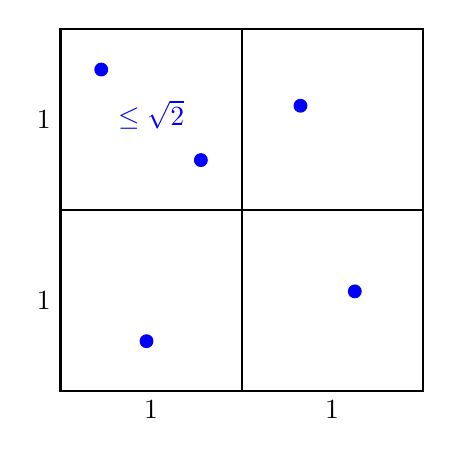
\begin{tikzpicture}[scale=1.15]
        \draw[thick] (0,0) rectangle (4,4);
        \draw[thick] (2,0) -- (2,4);
        \draw[thick] (0,2) -- (4,2);
        \node[below] at (1,0) {$1$};
        \node[below] at (3,0) {$1$};
        \node[left] at (0,1) {$1$};
        \node[left] at (0,3) {$1$};
        \filldraw[blue] (0.45,3.55) circle (2pt);
        \filldraw[blue] (1.55,2.55) circle (2pt);
        \filldraw[blue] (2.65,3.15) circle (2pt);
        \filldraw[blue] (3.25,1.10) circle (2pt);
        \filldraw[blue] (0.95,0.55) circle (2pt);
        \node[blue] at (1.0,3.05) {$\le \sqrt{2}$};
    \end{tikzpicture}
    \caption{Splitting a $2\times 2$ square into four $1\times 1$ squares.}
    \label{fig:square-four}
\end{figure}

A useful warning: drawing the points ``as far apart as possible'' can suggest the answer, but it is not a proof. The proof comes from forcing two points into the same small region whose diameter we can control.

\subsection*{Functions and Pigeonholes}

The Pigeonhole Principle can also be stated as a fact about functions.

\begin{theorem}
If $S$ and $T$ are finite sets and there exists an injective function $f:S\to T$, then $|S|\le |T|$.
Equivalently, if $|S|>|T|$, then there is no injective function from $S$ to $T$.
\end{theorem}

\begin{proof}
An injective function sends distinct elements of $S$ to distinct elements of $T$. Thus each element of $S$ must occupy its own separate image value in $T$. Therefore, $T$ must contain at least as many elements as $S$, so $|S|\le |T|$. The contrapositive says that if $|S|>|T|$, then some two elements of $S$ must be sent to the same element of $T$.
\end{proof}

In this language, the domain elements are the pigeons and the possible output values are the holes.

\subsection*{The Generalized Pigeonhole Principle}

The ordinary Pigeonhole Principle guarantees a repeated hole. The generalized version tells us how large some hole must be.

\begin{theorem}[Generalized Pigeonhole Principle]
Given $N$ objects and $k$ boxes, at least one box must contain at least
\[
    \left\lceil \frac{N}{k}\right\rceil
\]
objects.
\end{theorem}

\begin{proof}
Assume for contradiction that every box contains strictly fewer than $\left\lceil \frac{N}{k}\right\rceil$ objects. Since the number of objects in each box is an integer, each box contains at most
\[
    \left\lceil \frac{N}{k}\right\rceil -1
\]
objects. Therefore the total number of objects is at most
\[
    k\left(\left\lceil \frac{N}{k}\right\rceil -1\right).
\]
Since $\left\lceil \frac{N}{k}\right\rceil < \frac{N}{k}+1$, we get
\[
    k\left(\left\lceil \frac{N}{k}\right\rceil -1\right)
    < k\left(\frac{N}{k}+1-1\right)=N.
\]
So there are fewer than $N$ objects total, contradicting the assumption that there are $N$ objects. Hence some box contains at least $\left\lceil \frac{N}{k}\right\rceil$ objects.
\end{proof}

A common type of problem asks for the minimum number of objects needed to guarantee that at least $r$ of them land in the same one of $k$ boxes. The worst case is to place $r-1$ objects into each box without reaching $r$ in any box. This uses
\[
    k(r-1)
\]
objects. Therefore one more object forces some box to contain at least $r$ objects:
\[
    k(r-1)+1.
\]

\vspace{2mm}
\noindent\textbf{Example 3.} Given $100$ people, what is the minimum number of people who must have been born in the same month?

\begin{proof}
The pigeons are the $100$ people. The holes are the $12$ months. By the Generalized Pigeonhole Principle, some month contains at least
\[
    \left\lceil \frac{100}{12}\right\rceil = 9
\]
birthdays. Thus at least $9$ people were born in the same month.
\end{proof}

\vspace{2mm}
\noindent\textbf{Example 4.} In a meeting of six people, each pair is either friends or enemies. Show that there is a group of three people who are either all mutual friends or all mutual enemies.

\begin{proof}
Represent the six people as vertices of a complete graph. Color an edge red if the two corresponding people are friends, and blue if they are enemies.

\vspace{1.5mm}
Choose one person, call this person $A$. There are five edges coming out of $A$. Since each of these edges is either red or blue, the Pigeonhole Principle implies that at least three of them have the same color. Without loss of generality, suppose $A$ is connected by red edges to three people $B,C,D$.

\vspace{1.5mm}
Now look at the three edges among $B,C,D$: namely $BC$, $BD$, and $CD$.
\begin{itemize}
    \item If any of these edges is red, then that edge together with the two red edges from $A$ forms a red triangle. This gives three mutual friends.
    \item If none of these edges is red, then all three are blue. Thus $B,C,D$ form a blue triangle, giving three mutual enemies.
\end{itemize}
In all cases, there is a monochromatic triangle, so there are three people who are either all mutual friends or all mutual enemies.
\end{proof}

\begin{figure}[htbp]
    \centering
    \begin{subfigure}{0.45\textwidth}
        \centering
        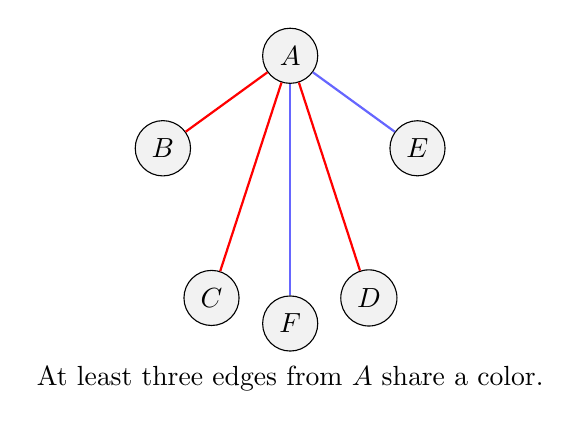
\begin{tikzpicture}[scale=1]
            \foreach \i/\name in {90/A,162/B,234/C,306/D,18/E,270/F} {
                \node[circle, draw, fill=gray!10, minimum size=7mm] (\name) at (\i:1.7) {$\name$};
            }
            \draw[red, thick] (A)--(B);
            \draw[red, thick] (A)--(C);
            \draw[red, thick] (A)--(D);
            \draw[blue!60, thick] (A)--(E);
            \draw[blue!60, thick] (A)--(F);
            \node at (0,-2.4) {At least three edges from $A$ share a color.};
        \end{tikzpicture}
    \end{subfigure}
    \begin{subfigure}{0.45\textwidth}
        \centering
        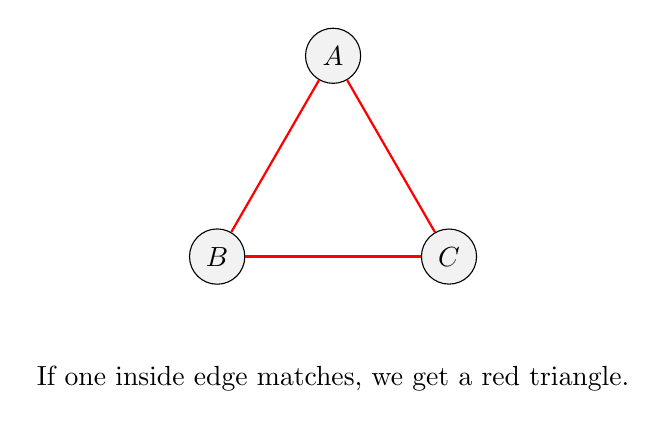
\begin{tikzpicture}[scale=1]
            \node[circle, draw, fill=gray!10, minimum size=7mm] (A) at (90:1.7) {$A$};
            \node[circle, draw, fill=gray!10, minimum size=7mm] (B) at (210:1.7) {$B$};
            \node[circle, draw, fill=gray!10, minimum size=7mm] (C) at (330:1.7) {$C$};
            \draw[red, thick] (A)--(B);
            \draw[red, thick] (A)--(C);
            \draw[red, thick] (B)--(C);
            \node at (0,-2.4) {If one inside edge matches, we get a red triangle.};
        \end{tikzpicture}
    \end{subfigure}
    \caption{The standard graph visualization of the six-person friendship/enmity problem.}
\end{figure}

\vspace{2mm}
\noindent\textbf{Example 5.}
\begin{enumerate}
    \item How many cards must be selected from a standard deck of $52$ cards to guarantee that at least three cards of the same suit are chosen?
    \item How many cards must be selected to guarantee that at least three hearts are selected?
\end{enumerate}

\begin{proof}
\begin{enumerate}
    \item The pigeons are the selected cards, and the holes are the four suits. We want to force some suit to contain at least $3$ cards. In the worst case, we can select $2$ cards from each of the $4$ suits without having three cards of any suit. That accounts for
    \[
        4\cdot 2=8
    \]
    cards. The next card forces some suit to appear for the third time. Therefore the answer is
    \[
        8+1=9.
    \]

    Equivalently, we need the smallest $N$ such that
    \[
        \left\lceil \frac{N}{4}\right\rceil \ge 3,
    \]
    which is $N=9$.

    \item This is different because the desired suit is fixed. We are not trying to force three cards of some suit; we are trying to force three hearts specifically.

    In the worst case, we first draw every non-heart card. There are $39$ non-hearts. After that, we must draw $3$ hearts to guarantee three hearts. Therefore the answer is
    \[
        39+3=42.
    \]
\end{enumerate}
\end{proof}
\noindent\textbf{Example 6.} Show that every sequence of $n^2+1$ distinct real numbers contains a subsequence of length $n+1$ that is either strictly increasing or strictly decreasing.

\begin{proof}
Let the sequence be
\[
    a_1,a_2,\dots,a_{n^2+1}.
\]
For each index $k$, define two numbers:
\begin{itemize}
    \item $I_k$: the length of the longest strictly increasing subsequence starting at $a_k$;
    \item $D_k$: the length of the longest strictly decreasing subsequence starting at $a_k$.
\end{itemize}
So each term $a_k$ receives a pair
\[
    (I_k,D_k).
\]

Assume for contradiction that there is no increasing or decreasing subsequence of length $n+1$. Then every increasing subsequence has length at most $n$, and every decreasing subsequence has length at most $n$. Hence
\[
    1\le I_k\le n
    \quad\text{and}\quad
    1\le D_k\le n
\]
for every $k$.

Therefore there are only $n^2$ possible pairs $(I_k,D_k)$. But there are $n^2+1$ terms in the sequence. By the Pigeonhole Principle, two indices $s<t$ must have the same pair:
\[
    (I_s,D_s)=(I_t,D_t).
\]

Now compare $a_s$ and $a_t$. Since the numbers are distinct, exactly one of the following holds.

\begin{Cases}
    \item $a_s<a_t$.

    Take a longest increasing subsequence starting at $a_t$. Since $s<t$ and $a_s<a_t$, we can place $a_s$ in front of that subsequence. This gives an increasing subsequence starting at $a_s$ of length $I_t+1$. Therefore
    \[
        I_s\ge I_t+1,
    \]
    contradicting $I_s=I_t$.

    \item $a_s>a_t$.

    Take a longest decreasing subsequence starting at $a_t$. Since $s<t$ and $a_s>a_t$, we can place $a_s$ in front of that subsequence. This gives a decreasing subsequence starting at $a_s$ of length $D_t+1$. Therefore
    \[
        D_s\ge D_t+1,
    \]
    contradicting $D_s=D_t$.
\end{Cases}

Both cases lead to contradictions. Therefore our assumption was false. Hence the sequence must contain either a strictly increasing subsequence of length $n+1$ or a strictly decreasing subsequence of length $n+1$.
\end{proof}

\section*{Post-Lecture}

\subsection*{Key Takeaways}

\begin{itemize}
    \item The Pigeonhole Principle proves that repetition is unavoidable when there are more objects than categories.
    \item The hard part is usually choosing the right pigeons and holes.
    \item Geometry problems often use regions as holes; the size of each region controls the maximum possible distance between two points in the same hole.
    \item Modular arithmetic problems often use congruence classes as holes.
    \item The generalized version says that among $N$ objects placed into $k$ boxes, some box contains at least $\left\lceil N/k\right\rceil$ objects.
    \item In ``minimum number to guarantee'' problems, build the worst-case arrangement that avoids the desired outcome, then add one more object.
\end{itemize}

\subsection*{Practice Problems}

\begin{enumerate}
    \item Show that among any $13$ people, at least two were born in the same month.
    \item Show that among any $367$ people, at least two have the same birthday, assuming birthdays are distributed among $366$ possible days.
    \item Show that among any $6$ integers, two have the same remainder modulo $5$.
    \item Show that among any $n+1$ integers, two differ by a multiple of $n$.
    \item A square of side length $3$ contains $10$ points. Show that two of the points are within distance $\sqrt{2}$ of each other.
\end{enumerate}

\end{document}
